\documentclass{report}
\usepackage{algorithmicx}
\usepackage{algorithm}
\usepackage{algpseudocode}
\usepackage{amsmath,amssymb,latexsym, mathtools}
\usepackage{changepage}
\usepackage{color}
\usepackage{enumerate}
\usepackage{fancyvrb}
\usepackage{float}
\usepackage{geometry}
\usepackage{inconsolata}
\usepackage{listings}
\usepackage{parskip}
\usepackage{subcaption}
\usepackage{tikz}
\usepackage{titlepic}
\usepackage{url}
\usepackage{verbatim}

\newcommand{\TODO}[1]{{\Huge TODO: #1}}
\newcommand{\algoref}[1]{Algorithm~\ref{alg:#1}}
\newcommand{\braced}[1]{\left[{#1}\right]}
\newcommand{\chapref}[1]{Chapter~\ref{chap:#1}}
\newcommand{\cpp}{C\texttt{++}}
\newcommand{\fftwomp}{\texttt{fftw\_omp}}
\newcommand{\figref}[1]{Figure~\ref{fig:#1}}
\newcommand{\fullomp}{\texttt{full\_omp}}
\newcommand{\icpc}{\texttt{icpc}}
\newcommand{\nbody}{$N$-body}
\newcommand{\partialomp}{\texttt{partial\_omp}}
\newcommand{\set}[1]{\left\{ {#1} \right\}}
\newcommand{\tabref}[1]{Table~\ref{tab:#1}}

% Fast Fourier Transform
\newcommand{\FFTsymbol}{\text{FFT}}
\newcommand{\FFT}[1]{\FFTsymbol\braced{#1}}
\newcommand{\invFFT}[1]{\FFTsymbol^{-1}\braced{#1}}

\definecolor{mygray}{rgb}{0.5,0.5,0.5}
\renewcommand\arraystretch{2}
\raggedbottom

 \lstset{ %
  %backgroundcolor=\color{white},   % choose the background color; you must add \usepackage{color} or \usepackage{xcolor}
  basicstyle=\footnotesize\ttfamily\linespread{0.8},        % the size of the fonts that are used for the code
  breakatwhitespace=false,         % sets if automatic breaks should only happen at whitespace
  breaklines=true,                 % sets automatic line breaking
  captionpos=b,                    % sets the caption-position to bottom
  commentstyle=\color{mygray},    % comment style
  deletekeywords={...},            % if you want to delete keywords from the given language
  escapeinside={\%*}{*)},          % if you want to add LaTeX within your code
  extendedchars=true,              % lets you use non-ASCII characters; for 8-bits encodings only, does not work with UTF-8
  frame=single,	                   % adds a frame around the code
  keepspaces=true,                 % keeps spaces in text, useful for keeping indentation of code (possibly needs columns=flexible)
  keywordstyle=\color{black},   % keyword style
  lineskip={-0.7pt},
  otherkeywords={*,...},            % if you want to add more keywords to the set
  numbers=left,                    % where to put the line-numbers; possible values are (none, left, right)
  numbersep=5pt,                   % how far the line-numbers are from the code
  %numberstyle=\tiny\color{mygray}, % the style that is used for the line-numbers
  rulecolor=\color{black},         % if not set, the frame-color may be changed on line-breaks within not-black text (e.g. comments (green here))
  showspaces=false,                % show spaces everywhere adding particular underscores; it overrides 'showstringspaces'
  showstringspaces=false,          % underline spaces within strings only
  showtabs=false,                  % show tabs within strings adding particular underscores
  stepnumber=2,                    % the step between two line-numbers. If it's 1, each line will be numbered
  %stringstyle=\color{mymauve},     % string literal style
  tabsize=2,	                   % sets default tabsize to 2 spaces
  title=\lstname                   % show the filename of files included with \lstinputlisting; also try caption instead of title
}

\setlength\parindent{0pt}

\begin{document}
\lstdefinestyle{nonumbers}
{numbers=none}

\title{Final Project Report\\~\\
	\large Parallel Particle-Mesh Methods Applied to the \nbody{} Problem}
\author{Michael Whittaker (mjw297)\\Sheroze Sheriffdeen (mss385)}
\titlepic{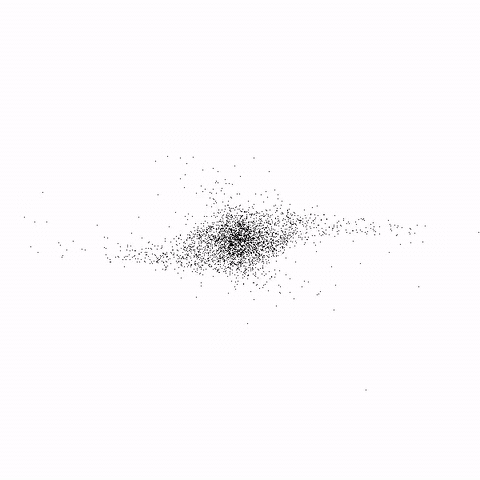
\includegraphics[width=0.7\textwidth]{./particles/9.png}}
\maketitle

% adjust margins to make table of contents fit on a single page
\newgeometry{left=1.5in, right=1.5in, top=1in, bottom=1in}
\tableofcontents
\restoregeometry

\chapter{Introduction}
This final project explores parallel particle-mesh methods applied to the collision-less \nbody{} problem in a shared memory programming model.

The \nbody{} system is a correlated dynamical system where each element can have a mass, radius, velocity, position and acceleration and each element is under the influence of a physical force, in our case, Newtonian gravity.

For the general \nbody{} problem with $N > 2$, barring selected configurations, the system cannot be solved analytically. To solve a system with $N > 2$, we create numerical models to approximate the evolution of the system with advancing time. Chapter~\ref{chap:models} introduces the physical and numerical models that enable us to simulate the behavior of bodies under the influence of gravity and discusses the performance and accuracy tradeoffs of the models.

Chapter~\ref{chap:impl} documents the implementation process of the simulation. The chapter presents a description and usage of the numerical libraries employed and the data marshaling and animation process.

Chapter~\ref{chap:perf} evaluates the performance of the system. The chapter analyzes the time profiles of the serial implementation and the parallel implementations, the strong and weak scaling properties of the parallel system and performance scaling with the number of particles and grid points.

Chapter~\ref{chap:sim} discusses a specific application of the \nbody{} simulator and the results of advancing a system of a large number of particles with time. This chapter introduces the correspondence between the simulation scales and the physical system and contains plots of the system evolution.

In conclusion, Chapter~\ref{chap:conc} mentions possible future work on the simulation and advanced numerical methods and parallelization schemes to further improve performance.


\chapter{Model Theory} \label{chap:models}

To simulate the \nbody{} problem, we have to employ models that enable us to track the attributes of the bodies of the system as we step forward in time. This section describes two such models and comments on their accuracy and performance tradeoffs.

\section{Particle-Particle Model} \label{sec:pp}
The first model of the \nbody{} problem is a particle-particle model. At each time step of the system, the velocity, position and acceleration attributes of an element need to be updated according to the following set of equations.
\begin{align}
	\dfrac{\vec{v_i}}{dt} &= \dfrac{\vec{F}_i}{m_i} = G \sum_{j \neq i} m_j \dfrac{\vec{x}_j - \vec{x}_i}{\vert \vec{x}_j - \vec{x}_i \vert^3} \\
	\dfrac{\vec{x}_i}{dt} &= \vec{v}_i
\end{align}

\noindent
where $m_i$ is the mass of the $i^{\text{th}}$ particle and $G$ is the gravitational constant. Given the acceleration vector acting on a particle, we can then use a time integration scheme to solve the above coupled set of equations. For example, we could use the automatic step Runge-Kutta method to update the position and velocity of each particle.

Although, this model provides good accuracy, the attributes modeled for a single element depend on every other elements in the system, leading to an algorithmic complexity of $O(N_p^2)$ where $N_p$ is the number of particles modeled by the system.

Therefore, for large number of particles we have to adopt a different model. Therefore, this project does not use the automatic stepsize Runge-Kutta method but further discussion of the method can be found in Chapter 17.2 of Numerical Recipes \cite{numrecipes}.

\section{Particle-Mesh Model}
In the particle-mesh approach, we exploit the force-at-a-point formulation and the field equation for the gravitational potential to compute a faster force calculation for the particles at the cost of accuracy. The space of interest is divided into a mesh and each particle is assigned to a mesh point depending on its location. The mesh sampling point defines the center of a cell.

\begin{figure}[H]
  \centering
  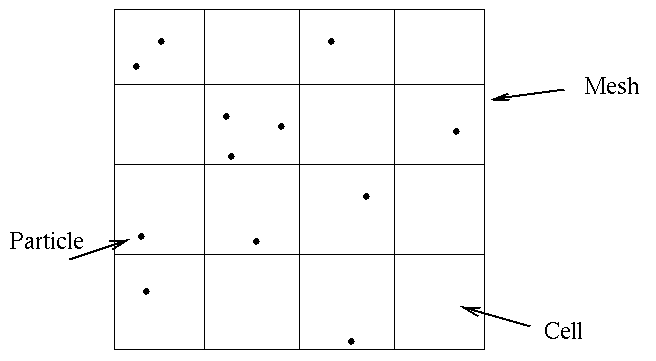
\includegraphics[scale=0.6]{pm_mesh.png}
  \caption{Particle-Mesh Model \cite{pm_mesh}}
   \label{fig:pm_mesh}
\end{figure}

\subsection{Physical Interpretation}

The gravitational field is defined at the center of a cell. Using the gravitational field at a mesh point, we can interpolate the force acting on a particle. To compute the gravitational field on a particle at a time step, we use Newton's law of universal gravitation:

\begin{equation}
	\dfrac{\vec{F}}{m} = \vec{g}
\end{equation}

The gravitational field $\vec{g}$ on a particle can be related to the gravitational potential $\phi$ by,

\begin{equation} \label{eq:phi_g}
	\vec{g} = - \nabla \phi
\end{equation}

and the potential $\phi(r)$ is related to the mass distribution by,

\begin{equation}
	\phi(r) = \dfrac{-Gm}{r}
\end{equation}

and obtaining the Poisson's equation for gravity:
\begin{equation}
	\nabla^2 \phi = 4\pi G \rho
\end{equation}

We can use Fourier analysis to solve the Poisson's equation for gravity. In Fourier space, the equation becomes,

\begin{equation} \label{eq:phi_k}
	k^2 \phi(\vec{k}) = 4 \pi G \rho(\vec{k})
\end{equation}

where $\vec{k}$ is the spatial frequency vector.

\subsection{Mass Density and the NGP scheme}

The mass density of the system is sampled at the cell centers of the mesh. To relate the masses of particles to the cell centers, a density assignment scheme is needed. The simplest method is the Nearest Grid Point (NGP) scheme.

\begin{equation}
	\rho_{i,j} = \dfrac{1}{(\Delta d)^2} \sum_{k=1}^{N_p} m_k \,
	\delta \left(\dfrac{x_k}{\Delta d} - i \right) \delta \left(\dfrac{y_k}{\Delta d} - j \right)
\end{equation}

where $\rho_{i,j}$ is the mass density at the cell $(i,j)$, $k$ iterates over the particles and $\Delta d$ is the sampling interval in space.

\algoref{ngp} describes the 2 dimensional NGP scheme on a square mesh where
$\text{cell}_{\rho}$ holds the mass density at the cell centers.

\begin{algorithm}[h]
  \begin{algorithmic}[1]
    \ForAll{particles $i$}
      \State find $(m, n)$: the index of the cell center in the mesh
      \State $\text{cell}_{\rho}(m,n) \gets \text{cell}_{\rho}(m,n) + m_i$
    \EndFor
    \ForAll{cell centers $(m, n)$}
      \State $\text{cell}_{\rho}(m,n) \leftarrow \text{cell}_{\rho}(m,n) / (\Delta d)^2$
    \EndFor
  \end{algorithmic}
  \caption{NGP scheme on square mesh}
  \label{alg:ngp}
\end{algorithm}

The NGP scheme provides a fast method to compute the mass distribution of the system since the core operation is a summation that runs in linear time proportional to the number of particles. The disadvantage of the NGP scheme is that the mass densities are discontinuous.

\subsection{Gravitational Potential and Acceleration}
To solve for the gravitational potential $\phi$, we obtained equation~\ref{eq:phi_k}. Using the NGP scheme, we obtain the spatial distribution of density. Converting this density distribution to Fourier space, we obtain the relationship,

\begin{align}
  \phi(\vec{k}) &= \dfrac{ 4 \pi G \cdot \FFT{\rho(x,y)} }{k^2} \\
  \phi(x,y) &= \invFFT{\dfrac{ 4 \pi G \cdot \FFT{\rho(x,y)}}{k^2}}
\end{align}

where $\FFTsymbol{}$ is the Fast Fourier Transform \cite{ngp}. The implementation details of $\FFTsymbol{}$ is described in Section~\ref{sec:fftw}.

Then, using equation~\ref{eq:phi_g}, we can solve for the gravitational acceleration at a cell center using the central difference method:

\begin{align}
	g_x(i,j) &= - \dfrac{\phi(i+1,j) - \phi(i-1, j)}{2 (\Delta d)} \\
	g_y(i,j) &= - \dfrac{\phi(i,j+1) - \phi(i, j-1)}{2 (\Delta d)}
\end{align}

The gravitational acceleration of the cell centers can now be associated with the particles in the simulation using the NGP scheme.

\subsection{Particle-Mesh Algorithm}
To summarize the particle-mesh method, \algoref{ppm} describes a single time step \cite{csup}.

\begin{algorithm}[h]
  \begin{algorithmic}[1]
    \State Assign mass to cell centers using the NGP scheme (\algoref{ngp}).
    \State Solve the Poisson's equation on the mesh in Fourier space by taking the Fourier transform of the mass distribution to obtain $\phi(\vec{k})$.
    \State Compute the inverse Fourier transform to obtain $\phi(x,y)$.
    \State Use central difference to obtain the gravitational acceleration at cell centers from $\phi(x,y)$.
    \State Use the NGP scheme to assign gravitational acceleration values to each particle.
    \State Use time integration to update the particle mass and velocity using the gravitational acceleration.
  \end{algorithmic}
  \caption{Particle-Mesh}
  \label{alg:ppm}
\end{algorithm}

\subsection{Performance and Accuracy tradeoffs}
The Particle-Particle model described in Section~\ref{sec:pp} although accurate requires a high computational cost, taking $O(N_p^2)$ time.

The advantage of the Particle-Mesh method is the performance. Updates to the particle attributes occur in $O(N_p)$ time. The slowest step in the method is the computation of the two dimensional Fourier transform which takes $O(N^2 \log(N^2))$ time.

The increase in performance comes with an accuracy cost. Using the NGP scheme to compute acceleration on a particle decreases the resolution of the solver and to obtain fairly accurate time integration, the spatial sampling interval should be smaller than the wavelengths of importance in the physical system. Finer mass interpolation schemes such as CIC and mixed schemes are discussed in Hockney and Eastwood's Computer simulation using particles \cite{csup}.

\chapter{Implementation}\label{chap:impl}
We have implemented a set of \nbody{} simulators using the Particle-Mesh model and algorithm in \cpp{} and a pair of simulation visualizers in Python. In this chapter, we discuss the implementation of both the simulators and visualizers.

\section{Simulators}\label{sec:simulator}
In this section, we first discuss FFTW: the fast Fourier transform library we use in our simulators. We then discuss the periodic boundary conditions we use in our algorithm. Finally, we discuss the implementation details of our simulators.

\subsection{FFTW}\label{sec:fftw}
To compute the Fourier transform required in the Particle-Mesh method, we use the Fast Fourier Transform, obtained from the FFTW package. (www.fftw.org, the "Fastest Fourier Transform in the West" \cite{fftw}). In FFTW, the Discrete Fourier Transform of a complex one dimensional array $X$ computes $Y$ where,

\begin{equation}
	Y_k = \sum_{j=0}^{n-1} X_j e^{-2 \pi j k i /n}
\end{equation}

In the solution implementation, to compute the Fourier space representation of the density distribution $\rho$, we perform a forward transform.

\begin{lstlisting}[aboveskip=11pt,belowskip=-10pt]
fftw_plan rho_plan =  fftw_plan_dft_r2c_2d(N, N, rho, rho_k, FFTW_MEASURE);
fftw_execute(rho_plan);
\end{lstlisting}

which takes \texttt{rho}, that holds $N \times N$ 2D samplings of $\rho(x, y)$ and stores the Fourier space representation in \texttt{rho\_k}.

The function \texttt{fftw\_plan\_dft\_r2c\_2d} creates a plan that binds two arrays to perform an FFT operation. \texttt{r2c} variants of this function denotes a transform that goes from real numbers to complex numbers.

To compute  $\phi$, we perform the computation in equation~\ref{eq:phi_k} and use an inverse transform to obtain $\phi(x,y)$.

\begin{lstlisting}[aboveskip=11pt,belowskip=-10pt]
fftw_plan phi_plan =  fftw_plan_dft_c2r_2d(N, N, rho_k, phi, FFTW_MEASURE);
fftw_execute(phi_plan);
\end{lstlisting}

Since we perform this FFT operation for multiple time steps, FFTW offers an option to analyze the fastest style of computation for the compute by passing in the \texttt{FFTW\_MEASURE} flag to the function.

\subsection{Periodic Boundary Conditions}
The Discrete Fourier Transform assumes periodic boundary conditions. Therefore, our 2D gravitational potential is implemented with a toroidal geometry:

\begin{align}
	\phi(x+L,y) &= \phi(x,y) \\
	\phi(x,y+L) &= \phi(x,y)
\end{align}

where $L$ is the side length of the simulation in physical units. Therefore, any particle that goes out of the grid is 'wrapped around' and introduced from the opposite end.

\begin{lstlisting}[aboveskip=11pt,belowskip=-10pt]
if (particle_pos[2*i] < 0.0) particle_pos[2*i]     = fmod(particle_pos[2*i], L) + L;
if (particle_pos[2*i] > L) particle_pos[2*i]       = fmod(particle_pos[2*i], L);
if (particle_pos[2*i+1] < 0.0) particle_pos[2*i+1] = fmod(particle_pos[2*i+1], L) + L;
if (particle_pos[2*i+1] > L) particle_pos[2*i+1]   = fmod(particle_pos[2*i+1],L);
\end{lstlisting}

\subsection{Serial Simulator}
Our serial simulator, found in \texttt{serial\_opt.cpp}, is a direct implementation of \algoref{ppm} which uses FFTW for the fast Fourier transforms. The serial simulator, as well as the other simulators, accepts a set of command line arguments that alter the execution of the simulation.
\begin{itemize}
  \item The \texttt{-l <$L$>} flag instructs our simulator to simulate on an
    underlying $L \times L$ space. By default particles are distributed
    uniformly at random with $x$ and $y$ coordinates between $\frac{2}{5}L$
    and $\frac{3}{5}L$.
  \item The \texttt{-n <$N$>} flag instructs our simulator to use an $N \times N$ mesh grid. The $N \times N$ grid is overlaid uniformly over the $L \times L$ space.
  \item The \texttt{-p <$N_p$>} flag instructs our simulator to simulate $N_p$ particles.
  \item The \texttt{-s <$s$>} flag instructs our simulator to perform $s$ time steps.
  \item The \texttt{-t <$\Delta t$>} flag instructs our simulator to use time step $\Delta t$.
\end{itemize}

\subsection{\fftwomp{} Simulator}
The \fftwomp{} simulator is the first of three parallel simulators and is found in \texttt{ppm\_omp.cpp}. The \fftwomp{} simulator is identical to the serial simulator except for one key difference: the fast Fourier transforms are done in parallel. FFTW provides parallel implementations of its fast Fourier transform functions that use OMP for parallelization, so this process is relatively easy. We simply add the following boilerplate to our serial simulator:

\begin{lstlisting}[aboveskip=11pt,belowskip=-10pt]
fftw_init_threads();                  // initialize FFTW for parallelization
fftw_plan_with_nthreads(num_threads); // set the number of OMP threads to use
// ...                                // plan and execute FFT's as usual
fftw_cleanup_threads();               // destroy threads
\end{lstlisting}

The \fftwomp{} simulator and the other two parallel simulators also accept a \texttt{-o $o$} flag which instructs the simulators to use $o$ OMP threads.

\subsection{\partialomp{} Simulator}
The \partialomp{} simulator, found in \texttt{ppm\_omp\_partial.cpp}, adds additional parallelization on top of the \fftwomp{} simulator. Specifically, it uses OMP to parallelize all loops that range over the particles. For example, consider the following loop found in the \fftwomp{} simulator which implements part of \algoref{ngp}:

\begin{minipage}{\linewidth}
\begin{lstlisting}[aboveskip=11pt,belowskip=-10pt]
int ind_x, ind_y, index, mass;
for (int i=0; i<N_p; i++) {
    ind_x =  floor(particle_pos[2*i]/delta_d);
    ind_y =  floor(particle_pos[2*i+1]/delta_d);
    index = ind_y*N + ind_x;
    mass = particle_mass[i];
    rho[index] += mass;
}
\end{lstlisting}
\end{minipage}

The \partialomp{} simulator parallelizes this loop with the \texttt{\#pragma omp parallel for} construct. It also protects shared memory accesses with appropriate mutual exclusion or atomic updates.

\begin{minipage}{\linewidth}
\begin{lstlisting}[aboveskip=11pt,belowskip=-10pt]
int ind_x, ind_y, index, mass;
#pragma omp parallel for                         // <-- new
for (int i=0; i<N_p; i++) {
    ind_x =  floor(particle_pos[2*i]/delta_d);
    ind_y =  floor(particle_pos[2*i+1]/delta_d);
    index = ind_y*N + ind_x;
    mass = particle_mass[i];
    #pragma omp critical                         // <-- new
    rho[index] += mass;
}
\end{lstlisting}
\end{minipage}

Note that the \partialomp{} simulator \emph{does not} parallelize all loops, only those that range over particles.

\subsection{\fullomp{} Simulator}
The \fullomp{} simulator, found in \texttt{ppm\_omp\_full.cpp}, builds off of the \partialomp{} simulator and very aggressively parallelizes \emph{all} loops. For example, consider the following loop which ranges over the $N \times N$ mesh. Since this loop does not range over the particles, the \partialomp{} simulator would not parallelize it, but the \fullomp{} simulator does.

\begin{minipage}{\linewidth}
\begin{lstlisting}[aboveskip=11pt,belowskip=-10pt]
#pragma omp for collapse(2) nowait
for (int j=0; j<N; j++) {
    for (int i=1; i<N-1; i++) {
        a_x[j*N + i] = (-phi[j*N + i-1] +  phi[j*N + i+1]) / scaling_factor;
    }
}
\end{lstlisting}
\end{minipage}

\section{Visualizers}
Our simulators iteratively updates the positions of the particles being simulated. After each iteration, it writes the particles' positions to a text file: a process known as marshalling. In addition to the positions, our simulator also marshals the size of the particle mesh ($N$), the number of particles ($N_p$), the number of iterations, and the masses of each particle. The marshalling logic is implemented in \texttt{marshaller.cpp}. Also note that our simulator only marshals data when debugging and is elided via conditional compilation otherwise.

The marshalled files are then parsed and animated by one of two visualizers.
The first, \texttt{scripts/mp4.py}, uses the MoviePy library \cite{moviepy} to
construct an MP4 visualization of the simulation. The second,
\texttt{scripts/gui.py}, uses the TkInter GUI library \cite{tkinter} to
animate the simulation in a GUI, without producing any output media files. Both visualizers also accept a set of command line options to modify the behavior of the simulation. For example, the \texttt{-f} flag sets the frames per second of the animation, and the \texttt{-p} flag sets the resolution of the animation.

Simulations with a large number of time steps or a large number of particles
can produce very large marshalled files. To alleviate the burden of storing and
transferring large files, the GUI visualizer can read and animate marshalled
data from the network rather than from a file. This allows us to animate
simulations without ever marshalling data to a file.

\chapter{Performance and Evaluation} \label{chap:perf}

In this chapter, we discuss how we used profiling to guide our optimization decisions, we discuss the tuning and optimizations we performed, and finally we evaluate the performance of our simulator with a large number of scaling studies.

\section{Profiling}
The first implementation of our particle simulator was naively implemented and single-threaded. By quickly writing a reference implementation of the simulator, we were able to quickly develop and debug our visualizers and check the correctness of our later optimized implementations. We also profiled the compilation and execution of our first implementation to guide our optimization efforts.

First, we examined the vectorization reports produced by \icpc{}. The reports showed that almost every one of our loops was being vectorized, not too surprising given the parallel nature of the Particle-Mesh algorithm. Moreover, the vectorization reports indicated that some of our arrays were unaligned. We vectorized the remaining of our loops and replaced invocations of \texttt{malloc} and \texttt{free} with invocations of \texttt{\_mm\_malloc} and \texttt{\_mm\_free} to align our arrays. After this, our vectorization reports showed fully vectorized loops with minor memory misalignment. A snippet of one of our vectorization reports is shown in \figref{vec-report}.

Next, we profiled the bottlenecks in the execution of our serial and parallel code using \texttt{amplxe-cl}, a snippet of which can be found in \figref{ampl}. The profiles show that the majority of the execution of our serial code is spent inside of the FFTW library. This is consistent with the Particle-Mesh algorithm which spends a considerable amount of time performing fast Fourier transforms. Moreover, this is desirable; the bottleneck of our code is in a library that has been \emph{very} thoroughly optimized. This means that we have successfully offloaded the bulk of the computation to a well-tuned library. The profiles report a similar pattern for our parallel code. The majority of the execution time is spent within the FFTW library. One notable difference is that the parallel code spends most of its time performing barrier operations to synchronize code. This suggested to us that increasing the number of threads would only improve the performance of the code given a large enough grid size. This hypothesis was confirmed by our scaling studies, as discussed later.

\begin{figure}[h]
  \centering
  \small
  \begin{BVerbatim}[gobble=4]
    LOOP BEGIN at common.cpp(57,5) inlined into serial_opt.cpp(78,9)
       remark #15388: vectorization support: reference rho_18337 has aligned access   [ common.cpp(58,9) ]
       remark #15388: vectorization support: reference rho_18337 has aligned access   [ common.cpp(58,9) ]
       remark #15399: vectorization support: unroll factor set to 4
       remark #15300: LOOP WAS VECTORIZED
       remark #15448: unmasked aligned unit stride loads: 1
       remark #15449: unmasked aligned unit stride stores: 1
       remark #15475: --- begin vector loop cost summary ---
       remark #15476: scalar loop cost: 35
       remark #15477: vector loop cost: 1.250
       remark #15478: estimated potential speedup: 13.440
       remark #15479: lightweight vector operations: 5
       remark #15488: --- end vector loop cost summary ---
    LOOP END
  \end{BVerbatim}
  \caption{A snippet of a vectorization report}
  \label{fig:vec-report}
\end{figure}

\begin{figure}[h]
  \centering
  \small
  \begin{minipage}{0.5\linewidth}
    \begin{BVerbatim}[gobble=4]
      Function        Module        CPU Time
      --------------  ------------  --------
      main            serial_opt      6.907s
      n1bv_64         serial_opt      3.855s
      n2fv_64         serial_opt      2.387s
      n1fv_32         serial_opt      1.808s
      hc2cbdftv_16    serial_opt      1.120s
      __intel_memset  serial_opt      1.100s
      hc2cfdftv_16    serial_opt      0.960s
      fftw_cpy1d      serial_opt      0.940s
      t2fv_32         serial_opt      0.900s
      fftw_cpy2d      serial_opt      0.898s
      t2bv_16         serial_opt      0.749s
    \end{BVerbatim}
  \end{minipage}%
  \begin{minipage}{0.5\linewidth}
    \begin{BVerbatim}[gobble=4]
      Function             Module              CPU Time
      -------------------  ------------------  --------
      __kmp_fork_barrier   libiomp5.so         283.260s
      n2fv_64              ppm_omp              13.749s
      n1bv_128             ppm_omp              12.812s
      n1bv_64              ppm_omp               9.395s
      main                 ppm_omp               7.493s
      hc2cbdftv_8          ppm_omp               5.470s
      n1fv_32              ppm_omp               4.710s
      fftw_cpy1d           ppm_omp               4.427s
      __kmp_launch_thread  libiomp5.so           3.570s
      hc2cfdftv_16         ppm_omp               2.587s
      __kmp_join_call      libiomp5.so           2.354s
    \end{BVerbatim}
  \end{minipage}
  \caption{A snippet of an \texttt{amplxe-cl} profile for our serial code (left) and parallel code (right)}
  \label{fig:ampl}
\end{figure}

\section{Optimizations}
One benefit of the Particle-Mesh algorithm is that majority of the complexity and runtime is taken by the fast Fourier transforms. By leveraging the FFTW library to perform these transforms, our algorithm gets a heavily optimized kernel for free! Still, we performed a variety of optimizations to further improve the performance of our simulators.

\begin{itemize}
  \item We compiled our simulators with the \texttt{-O3} \texttt{-no-prec-div}, \texttt{-ipo}, \texttt{-restrict}, and \texttt{-xCORE-AVX2} \icpc{} compiler flags. This provided a quick and easy speedup for all our simulators.
  \item We download, configure, build, and install the FFTW libraries from scratch on the totient cluster. By default, FFTW is built with \texttt{gcc} and does not include some optimizations. We configured FFTW to build with \texttt{icc} and we enabled vectorization during its compilation. This sped up all our simulators significantly.
  \item As discussed in above, we vectorized every loop in our simulators and aligned memory with calls to \texttt{\_mm\_malloc}.
  \item The FFTW library plan generation function accepts a flag that is either \texttt{FFTW\_ESTIMATE} or \texttt{FFTW\_MEASURE}. When \texttt{FFTW\_ESTIMATE} is specified, FFTW estimates a reasonable execution plan. If \texttt{FFTW\_MEASURE} is specified, then FFTW performs a set of experiments to determine which execution plan is likely to be optimal. Since we generate an execution plan once and re-use it for every iteration of the simulation, we make sure to initialize plans with the \texttt{FFTW\_MEASURE} flag.
  \item We made sure to avoid certain pitfalls when using OMP in our \partialomp{} and \fullomp{} simulators. For example, we use a single \texttt{\#pragma omp parallel} construct and multiple \texttt{\#pragma omp for} constructs in our \fullomp{} simulator rather than using multiple \texttt{\#pragma omp parallel for}. We also use \texttt{\#pragma omp atomic} rather than \texttt{\#pragma omp critical} when possible. Finally, we use the \texttt{nowait} specifier whenever possible to avoid barrier overheads.
\end{itemize}

\section{Scaling Studies}
In this section, we perform a large number of scaling studies to thoroughly evaluate the performance and scalability of our particle simulator. \figref{timevsthreads}, \figref{speedupvsthreads}, \figref{weak}, \figref{timevsna}, \figref{timevsnb}, \figref{speedupvsna}, \figref{speedupvsnb}, and \figref{timevsp} present the data gathered during our experiments.

\subsection{Strong Scaling Study}
We conducted a strong scaling study to measure the scalability of our implementations. We fixed the number of particles at $N_p = 12800$. Then, for each grid size ($N$) in $\set{128, 256, 512, 1024, 2048, 4096}$, we executed our particle simulators for 1, 2, 3, 4, 5, 6, 7, 8, 12, 16, 20, and 24 threads. \figref{timevsthreads} charts the average iteration execution time; \figref{speedupvsthreads} charts the average speedup compared to our serial implementation.

The strong scaling study provides a number of interesting insights. First, for small $N$, increasing the number of threads never decreases and sometimes increases the execution time of the simulators. This is consistent with our intuition and consistent with the profiles presented in \figref{ampl}. When the grid is too small, there is simply not enough work for a large number of threads. As a result, the majority of the execution time is spent synchronizing threads. On the other hand, for large $N$, increasing the number of threads does significantly improve the performance of the code. Notably, for $N=2048$ and $N = 4096$, the \fftwomp{} and \partialomp{} simulators execute almost twice as fast as our serial implementation. We hypothesize that for even larger grids, and for fewer particles, the speedup will continue to increase. Of course, these results are not surprising. The FFTW documentation even reports that ``if the problem size is too small, you may want to use fewer threads than you have processors'' \cite{fftwthreads}.

The scaling study also shows the relative performance of the \fftwomp{}, \fullomp{}, and \partialomp{} simulators. For small values of $N$, the \partialomp{} and \fullomp{} simulators perform similarly and both perform worse than the \fftwomp{} simulator. When $N$ increases, the performance of the \partialomp{} simulator approaches that of the \fftwomp{} simulator, and the performance of the \fullomp{} simulator decreases. This can again be attributed to thread synchronization overhead. The \fullomp{} simulator aggressively parallelizes loops over the grid, and some of these loops have critical sections within them. As the grid size increases, the overhead of synchronizing threads within the loop outweighs the benefits of parallelizing the loop to start with. Moreover, the fact that the \fftwomp{} and \partialomp{} simulator converge in performance suggests that for large grid sizes and a modest number of particles, the majority of the time is spent performing fast Fourier transforms and not on particle processing. This is again consistent with the profiles presented in \figref{ampl} and is confirmed by our particle scaling experiments discussed below.

\subsection{Weak Scaling Study}
We also performed a weak scaling study to measure the scalability of our simulators. For each number of threads $o$ in $\set{1, 2, 3, 4, 5, 6, 7, 8, 12, 16, 20, 24}$, we selected a grid size $N_o$ such that each thread has an equal amount of work. Since the running time of the Particle-Mesh algorithm is bounded by the fast Fourier transformation, there is $O(N_o^2 \log(N_o^2))$ work. Thus, we find $N_o$ by solving the following equation for all $o$ where $k$ is a constant.
\begin{equation}
  \frac{N_o^2 \log(N_o^2)}{t} = k
\end{equation}
We let $N_1 = 256$, so $k = 256^2 \log(256^2)$. We then solved for $N_o$ numerically, the values of which are reported in \tabref{no}.

\begin{table}[ht]
  \centering
  \begin{tabular}{|c|c|c|c|c|c|c|c|c|c|c|c|c|}
    \hline
    $o$  &1  &2  &3  &4  &5  &6  &7  &8  &12 &16 &20 &24   \\\hline
    $N_o$&256&352&424&485&538&585&628&669&807&923&1024&1115\\\hline
  \end{tabular}
  \caption{$N_o$ for $o \in \set{1, 2, 3, 4, 5, 6, 7, 8, 12, 16, 20, 24}$}
  \label{tab:no}
\end{table}

Then, we varied the number of particles in the set $N_p = \set{1600, 3200, 6400, 12800}$, and measured the average time step execution time for each of our simulators. We scaled each execution time by the execution time of the single threaded case to compute efficiency. This is charted in \figref{weak}. The weak scaling study shows a decrease in efficiency as we increase the number of threads. This is expected and caused by the overheads of synchronizing threads. Moreover, the results are consistent with the results of the strong scaling study and show that the \fftwomp{} and \partialomp{} simulators perform similarly, while the \fullomp{} simulator is generally less efficient.

\subsection{Grid Size Scaling}
In addition to strong and weak scaling studies, we also measured the performance of our simulators with respect to grid size for a varying number of threads. The data---presented in \figref{timevsna}, \figref{timevsnb}, \figref{speedupvsna}, and \figref{speedupvsnb}--- is similar to the data found in the strong scaling study. \figref{timevsna} and \figref{timevsnb} confirm the $N^2\log(N^2)$ runtime of the Particle-Mesh algorithm. They also confirm that the \fullomp{} simulator performs worse than the other two simulators, no matter the number of threads. The data also makes it clear that the \fftwomp{} and \partialomp{} simulators have very similar performance. \figref{speedupvsna} and \figref{speedupvsnb} show an alternate view of the same data. Most importantly, they highlight the fact that the \fftwomp{} and \partialomp{} simulators perform almost twice as well as the serial implementation for large $N$.

\subsection{Particle Scaling}
As discussed in \chapref{impl}, \fftwomp{} invokes a parallelized implementation of FFTW's fast Fourier transform function; the \partialomp{} simulator introduces additional parallelization by parallelizing loops ranging over particles; and the \fullomp{} simulator additionally parallelizes all loops. Our previous scaling studies show that \fullomp{} is too aggressive and has poor performance because of its heavy synchronization overhead. Our \partialomp{} simulator has less overhead because it only parallelizes loops over the particles. If the number of particles is large, it's possible that the parallelization benefits outweigh the synchronization overhead. We performed a scaling study with respect to the number of particles to explore this hypothesis. We fixed a small grid size of $N = 128$ and benchmarked the performance of our simulators for 1, 2, 3, and 4 threads. The data is presented in \figref{timevsp}.

The data shows that for all three simulators, increasing the number of threads decreases the performance of the simulators for all number of particles. These results are again confirmed by the profile in \figref{ampl}. The bottleneck of our simulators is in FFTW, not in particle processing. This means that if we fix a small grid size of $N=128$ so that additional threads do not increase the performance of the fast Fourier transform, then adding more threads does not significantly help process the particles. In other words, adding more threads doesn't help particle processing. It's possible that if we increase the number of particles by one or two orders of magnitude, that multiple threads could begin to be beneficial, but given an enormous amount of particles, it becomes practical to increase the grid size to maintain a decent level of accuracy. When we increase the grid size though, the overhead of FFTW increasingly dominates the cost of particle processing. Thus, it is unclear that parallelization will ever benefit particle processing, no matter the number of particles.

% filename 1
% caption 1
% label 1
% filename 2
% caption 2
% label 2
\newcommand{\sidebyside}[6]{
  \makebox[\textwidth][c]{
    \begin{subfigure}[c]{0.5\textwidth}
      \centering
      \includegraphics[width=\textwidth]{#1}
      \caption{#2}
      \label{fig:#3}
    \end{subfigure}
    \quad
    \begin{subfigure}[c]{0.5\textwidth}
      \centering
      \includegraphics[width=\textwidth]{#4}
      \caption{#5}
      \label{fig:#6}
    \end{subfigure}
  }
}

\newcommand{\timevsthreads}[1]{figs/time_vs_num_threads-N=#1.pdf}
\newcommand{\speedupvsthreads}[1]{figs/speedup_vs_num_threads-N=#1.pdf}
\newcommand{\timevsn}[1]{figs/time_vs_N-t=#1.pdf}
\newcommand{\speedupvsn}[1]{figs/speedup_vs_N-t=#1.pdf}
\newcommand{\timevsp}{figs/time_vs_p.pdf}

\newgeometry{left=1in, right=1in, top=1in, bottom=1in}
\begin{figure}[h]
  \centering
  \foreach \x/\y in {128/256, 512/1024, 2048/4096} {
    \sidebyside{\timevsthreads{\x}}{}{timevsthreads-\x}
               {\timevsthreads{\y}}{}{timevsthreads-\y}
  }
  \caption{Average iteration time vs number of threads}
  \label{fig:timevsthreads}
\end{figure}

\begin{figure}[h]
  \centering
  \foreach \x/\y in {128/256, 512/1024, 2048/4096} {
    \sidebyside{\speedupvsthreads{\x}}{}{speedupvsthreads-\x}
               {\speedupvsthreads{\y}}{}{speedupvsthreads-\y}
  }
  \caption{Speedup vs number of threads}
  \label{fig:speedupvsthreads}
\end{figure}

\begin{figure}[h]
  \centering
  \foreach \x/\y in {1/2, 3/4, 5/6} {
    \sidebyside{\timevsn{\x}}{}{timevsn-\x}
               {\timevsn{\y}}{}{timevsn-\y}
  }
  \caption{Average iteration time vs grid size ($N$)}
  \label{fig:timevsna}
\end{figure}
\begin{figure}[h]
  \centering
  \foreach \x/\y in {7/8, 12/16, 20/24} {
    \sidebyside{\timevsn{\x}}{}{timevsn-\x}
               {\timevsn{\y}}{}{timevsn-\y}
  }
  \caption{Average iteration time vs grid size ($N$)}
  \label{fig:timevsnb}
\end{figure}

\begin{figure}[h]
  \centering
  \foreach \x/\y in {1/2, 3/4, 5/6} {
    \sidebyside{\speedupvsn{\x}}{}{speedupvsn-\x}
               {\speedupvsn{\y}}{}{speedupvsn-\y}
  }
  \caption{Speedup vs grid size ($N$)}
  \label{fig:speedupvsna}
\end{figure}
\begin{figure}[h]
  \centering
  \foreach \x/\y in {7/8, 12/16, 20/24} {
    \sidebyside{\speedupvsn{\x}}{}{speedupvsn-\x}
               {\speedupvsn{\y}}{}{speedupvsn-\y}
  }
  \caption{Speedup vs grid size ($N$)}
  \label{fig:speedupvsnb}
\end{figure}

\begin{figure}[h]
  \centering
  \includegraphics[width=\textwidth]{\timevsp}
  \caption{Average iteration time vs number of particles ($N_p$)}
  \label{fig:timevsp}
\end{figure}
\restoregeometry


\chapter{Simulation Results} \label{chap:sim}

To see the \nbody{} simulation in action, we model a distribution of bodies with a mean mass of one solar mass around a massive object at the center.

\section{Conversion Units}

To scale the floating point numbers of the simulation, we adopt the following conversion units \cite{conversion}.

\begin{center}
  \begin{tabular}{| l | l |}
    \hline
    \textbf{Simulation Units} & \textbf{Physical Units} \\ \hline
    Time unit ($\Delta t$ = 1) & 1 year ($3.15 \times 10^7$ seconds)\\
    Space unit ($\Delta d$ = 1) & 1 AU ($1.4960 \times 10^{11}$ meters) \\
    Mass unit ($\Delta m$ = 1) & 1 solar mass ($1.9891 \times 10^{30}$ kilograms) \\ \hline
  \end{tabular}
\end{center}

\section{Initial Conditions}

\subsection{Space distribution}

The simulation space is an $L \times L$ torus. The positions of the particles are randomly distributed according to a bivariate Gaussian distribution. The positions are sampled from the distributions,

\begin{align}
	p_x &= \dfrac{1}{\sqrt{2 \pi} \sigma} \exp{ -\frac{(x - \mu_x)^2}{2 \sigma^2}} \\
	p_y &= \dfrac{1}{\sqrt{2 \pi} \sigma} \exp{ -\frac{(y - \mu_y)^2}{2 \sigma^2}}
\end{align}

where $\mu_x = \mu_y = \dfrac{L}{2}$. This sampling produces particles that are centered around $\left( \dfrac{L}{2}, \dfrac{L}{2} \right)$ where a massive particle with mass $1000M_{\odot}$ lies. The bodies form a ``bulge'' around the center of the configuration.

\subsection{Mass distribution}

Masses of the particles, excepting the central mass, are Poisson distributed with an expected value $\lambda$ of 1 solar mass.
\begin{equation}
	p_m = \dfrac{\lambda^k}{k!} e^{-\lambda} \quad\quad \text{where $k \in \{0, 1, 2, 3, \ldots\}$}
\end{equation}

\subsection{Velocity distribution}

The initial velocities of the particles are assigned assuming a stable circular orbit around the central mass neglecting the surrounding particles.
\begin{align}
	v_x &= -\sin(\theta) \sqrt{\dfrac{GM}{r}}\\
	v_y &= \cos(\theta) \sqrt{\dfrac{GM}{r}}
\end{align}

where $M$ is the mass of the central body, $G$ is the gravitational constant, $r$ is the separation between the central mass and the particle, and $\theta$ is the azimuthal angle between the central body and the particle body where the central body is at the origin. This provides the initial rotational component for the galaxy but does not create a stable configuration.

\subsection{Time Evolution Plots}

Given the initial conditions as described above, with simulation side length of $60$AU, 3000 particles, and a time step of $0.86$ hours, we advance the simulation and plot the resulting particle configuration at specific time intervals. The complete simulation can be found in \texttt{particles.gif}.

\begin{figure}[H]
     	\centering
	\begin{subfigure}{.48\textwidth}
	\centering
     	\fbox{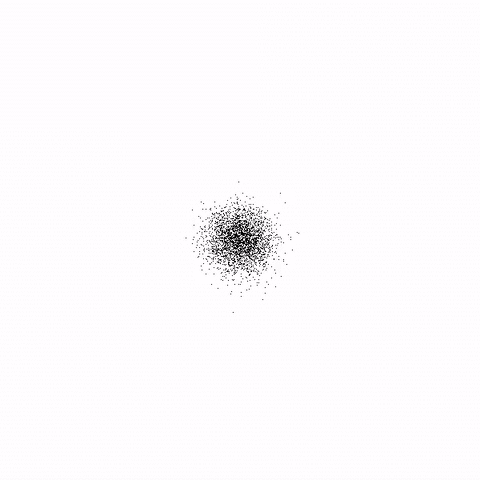
\includegraphics[width=0.95\linewidth]{./particles/0.png}}
	\caption{Bodies at $t = 0.0$ days, $L = 60$AU}
	\end{subfigure}
	\begin{subfigure}{.48\textwidth}
	\centering
     	\fbox{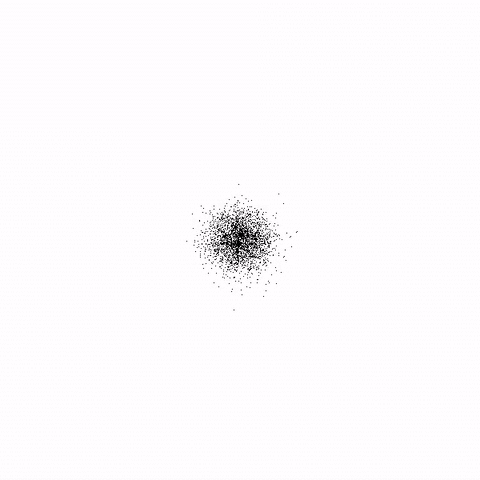
\includegraphics[width=0.95\linewidth]{./particles/1.png}}
	\caption{Bodies at $t = 2.43$ days, $L=60$AU}
	\end{subfigure}
	\begin{subfigure}{.48\textwidth}
	\centering
     	\fbox{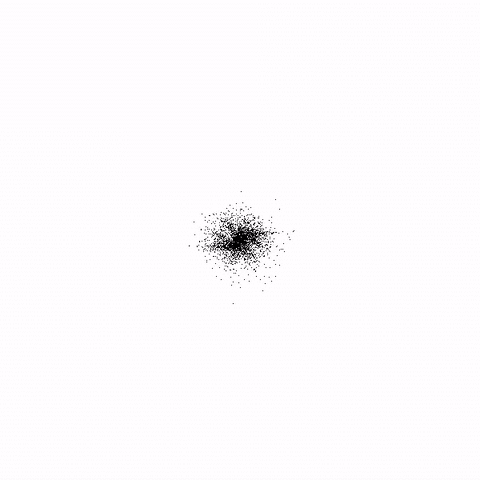
\includegraphics[width=0.95\linewidth]{./particles/2.png}}
	\caption{Bodies at $t = 4.86$ days, $L=60$AU}
	\end{subfigure}
	\begin{subfigure}{.48\textwidth}
	\centering
     	\fbox{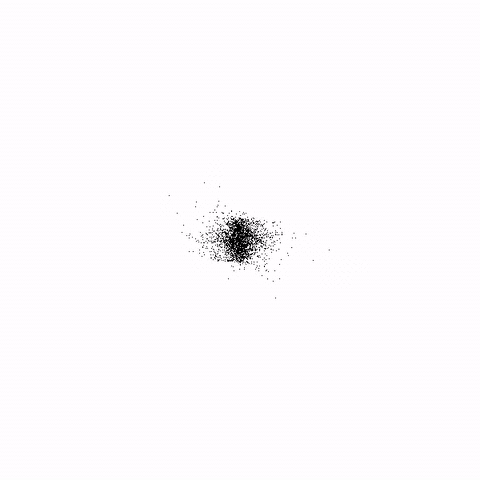
\includegraphics[width=0.95\linewidth]{./particles/4.png}}
	\caption{Bodies at $t = 7.3$ days, $L=60$AU}
	\end{subfigure}
	\caption{Configuration evolution with $\Delta t= 0.86$ hours, 3000 particles, $\mu_m = 1 \times 10^{30}$ kg}
	\label{fig:ev0}
\end{figure}

\begin{figure}[H]
     	\centering
	\begin{subfigure}{.48\textwidth}
	\centering
     	\fbox{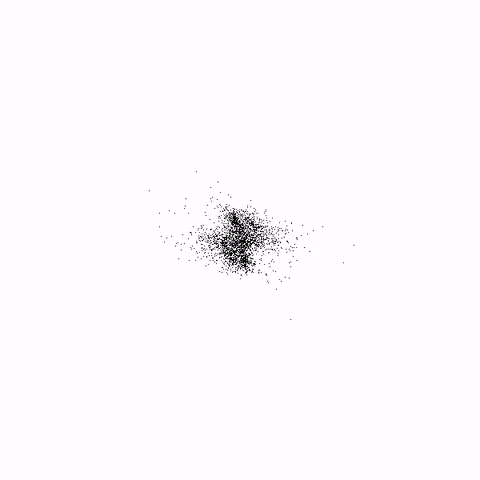
\includegraphics[width=0.95\linewidth]{./particles/5.png}}
	\caption{Bodies at $t = 9.73$ days, $L=60$AU}
	\end{subfigure}
	\begin{subfigure}{.48\textwidth}
	\centering
     	\fbox{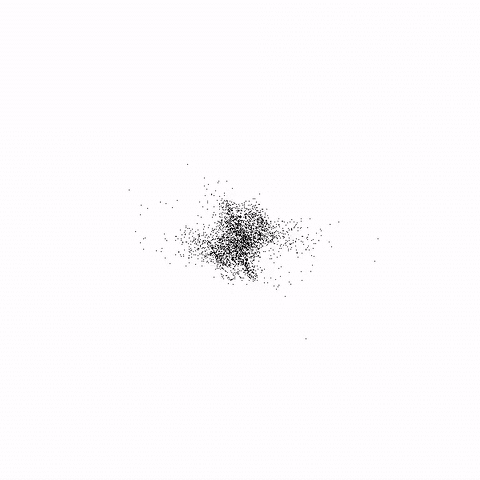
\includegraphics[width=0.95\linewidth]{./particles/6.png}}
	\caption{Bodies at $t = 12.16$ days, $L=60$AU}
	\end{subfigure}
	\begin{subfigure}{.48\textwidth}
	\centering
     	\fbox{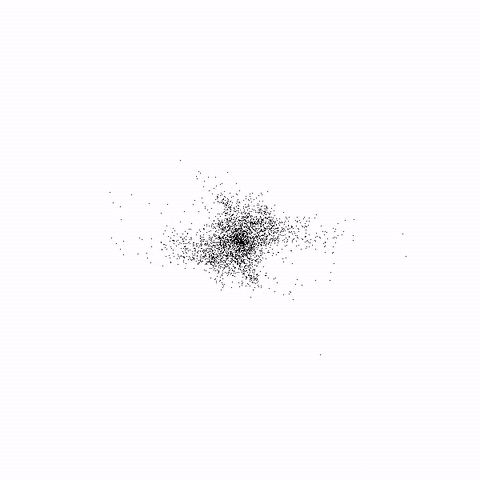
\includegraphics[width=0.95\linewidth]{./particles/7.png}}
	\caption{Bodies at $t = 14.6$ days, $L=60$AU}
	\end{subfigure}
	\begin{subfigure}{.48\textwidth}
	\centering
     	\fbox{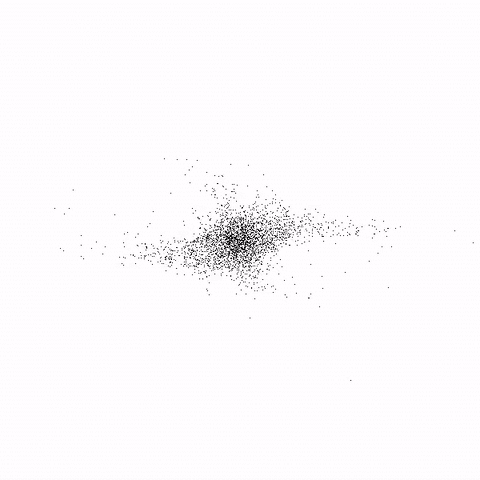
\includegraphics[width=0.95\linewidth]{./particles/8.png}}
	\caption{Bodies at $t = 17.03$ days, $L=60$AU}
	\end{subfigure}
	\caption{Configuration evolution with $\Delta t= 0.86$ hours, 3000 particles, $\mu_m = 1 \times 10^{30}$ kg}
	\label{fig:ev1}
\end{figure}

\begin{figure}[H]
     	\centering
	\begin{subfigure}{.48\textwidth}
	\centering
     	\fbox{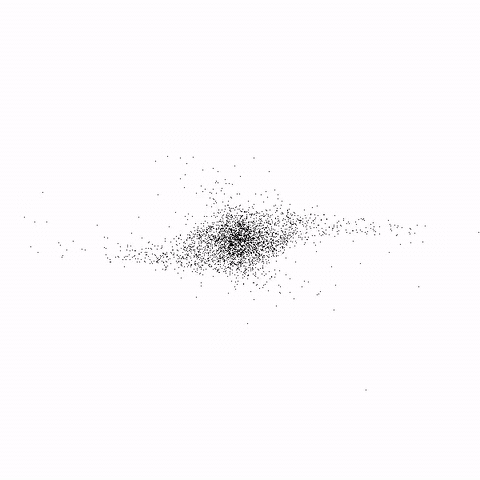
\includegraphics[width=0.95\linewidth]{./particles/9.png}}
	\caption{Bodies at $t = 19.46$ days, $L=60$AU}
	\end{subfigure}
	\begin{subfigure}{.48\textwidth}
	\centering
     	\fbox{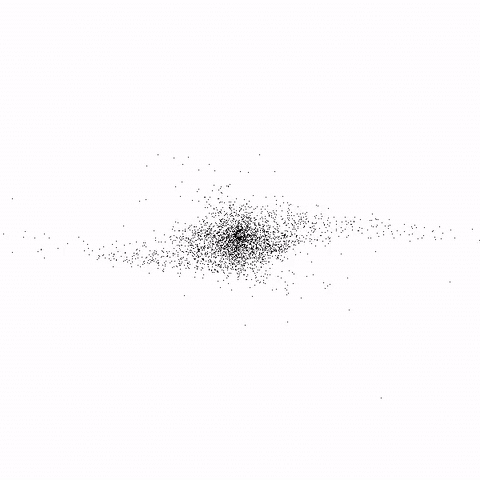
\includegraphics[width=0.95\linewidth]{./particles/10.png}}
	\caption{Bodies at $t = 21.9$ days, $L=60$AU}
	\end{subfigure}
	\begin{subfigure}{.48\textwidth}
	\centering
     	\fbox{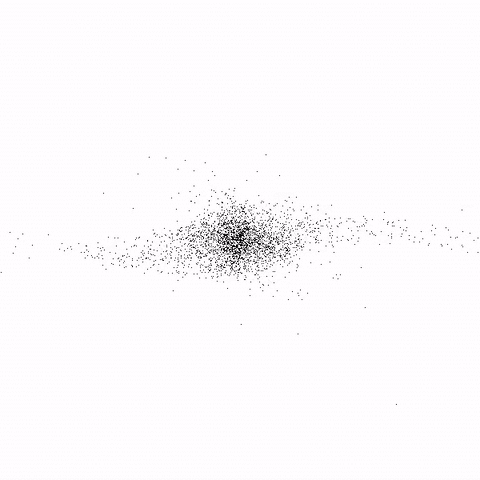
\includegraphics[width=0.95\linewidth]{./particles/11.png}}
	\caption{Bodies at $t = 24.33$ days, $L=60$AU}
	\end{subfigure}
	\begin{subfigure}{.48\textwidth}
	\centering
     	\fbox{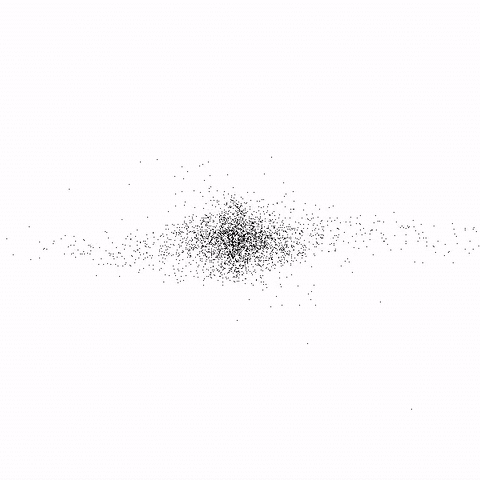
\includegraphics[width=0.95\linewidth]{./particles/12.png}}
	\caption{Bodies at $t = 26.76$ days, $L=60$AU}
	\end{subfigure}
	\caption{Configuration evolution with $\Delta t= 0.86$ hours, 3000 particles, $\mu_m = 1 \times 10^{30}$ kg}
	\label{fig:ev2}
\end{figure}

\chapter{Conclusion} \label{chap:conc}
To improve the time integration process, future work can be undertaken to automatically scale the time step size to prevent instabilities. A maximum velocity can be enforced on the mesh, proportional to the cell widths, to limit the information propagation rate across the cells and the next time step can be dilated accordingly.

A better approximation for mass assignments to cells than the NGP scheme discussed here is the CIC method or the "cloud-in-cell" method described in Chapter 5-2-3 of Hockney and Eastwood's Computer simulation using particles \cite{csup}. It is costlier in terms of floating point operations per mass assignment run, but provides a more accurate estimate, giving forces continuous in volume. This method considers the closest $2^N$ neighbors where $N$ is the dimensionality of the problem, to assign masses.

The biggest shortcoming of the Particle-Mesh method is the low resolution of forces computed when particles are near each other. This arises from the regular discretization scheme and is proportional to the cell width $\Delta d$. To overcome this shortcoming, a possible numerical model is the P3M model \cite{ngp}. The Particle-Particle/Particle-Mesh model refines the mesh method by computing the pair-wise force interaction between particles if the distance between particles are below a certain threshold. P4M method is a parallel variant of the P3M and improves on the performance \cite{p4m}.

To scale the \nbody{} simulation to large values, a smarter scheme is needed that is able to distribute the computation across multiple computers. OpenMP, due to its shared memory programming model, does not provide this ability to scale. MPI does enable us to perform computations in parallel on separate processors that can span multiple machines. FFTW offers an MPI variant of the FFT computation that can be used to explore the distributed computation model \cite{fftw_mpi}.

\begin{thebibliography}{9}
\bibitem{numrecipes}
W. H. Press, S. A, Teukolsky, W. T. Vetterling and B. P. Flannery
\textit{Numerical Recipes, The Art of Scientific Computing, 3rd Edition}.
Camb. Univ. Press 2007.

\bibitem{csup}
R. Hockney, J. Eastwood, \textit{Computer simulation using particles} (Special student ed.). Bristol [England: A. Hilger.(1988)

\bibitem{dawson}
J. Dawson. \textit{Reviews of Modern Physics} 55, p.403 (1983)

\bibitem{pm_mesh}
M. Elmohamed (n.d.). \textit{N-Body Simulations}. Retrieved December 13, 2015, from http://www.new-npac.org/projects/cdroms/cewes-1999-06-vol2/cps615course/nbody-materials/nbody-simulations.html

\bibitem{ngp}
F. Vesely (n.d.). \textit{9.2 Particle-Mesh Methods (PM and P3M)}:. Retrieved December 13, 2015, from http://homepage.univie.ac.at/franz.vesely/simsp/dx/node48.html

\bibitem{fftw}
M. Frigo, S. G. Johnson, \textit{Design and Implementation of FFTW3}, Proc. of the IEEE, 93
(2005), p. 216-231.

\bibitem{moviepy}
\textit{MoviePy User Guide}. (n.d.). Retrieved December 14, 2015, from https://zulko.github.io/moviepy/

\bibitem{tkinter}
\textit{TkInter Documentation}. (n.d.). Retrieved December 14, 2015, from https://wiki.python.org/moin/TkInter

\bibitem{conversion}
C. Mihos. (n.d.). \textit{Spiral Galaxies}. Retrieved December 14, 2015, from http://burro.case.edu/Academics/Astr222/equations.pdf

\bibitem{nbody_cmu}
\textit{N-Body/Particle Simulation Methods}. (n.d.). Retrieved December 14, 2015, from https://www.cs.cmu.edu/afs/cs/academic/class/15850c-s96/www/nbody.html

\bibitem{p4m}
P. Brieu, A. Evrard. (2000). \textit{P4M: A parallel version of P3M}. In New Astronomy (3rd ed., Vol. 5, pp. 163-180). Elsevier.

\bibitem{fftw_mpi}
\textit{Distributed-memory FFTW with MPI}. (n.d.). Retrieved December 14, 2015, from \url{http://fftw.org/doc/Distributed_002dmemory-FFTW-with-MPI.html}

\bibitem{git}
S. Sheriffdeen, M. Whittaker, (n.d.). \textit{Parallel Particle Mesh applied to \nbody{} simulations}. Retrieved December 14, 2015, from https://github.com/sheroze1123/ppm

\bibitem{vect}
Intel\textregistered  Xeon Phi\texttrademark Coprocessor - the Architecture. (n.d.). Retrieved December 14, 2015, from https://software.intel.com/en-us/articles/intel-xeon-phi-coprocessor-codename-knights-corner

\bibitem{openmp}
B. Barney (n.d.). \textit{OpenMP Tutorial}. Retrieved December 14, 2015, from https://computing.llnl.gov/tutorials/openMP/

\bibitem{astroparticle}
\textit{Solving the collisionless Boltzmann equation using \nbody{} simulations}. (n.d.). Retrieved December 14, 2015, from http://www.mi.infn.it/isapp04/Moore/notes2.pdf

\bibitem{simd}
G. Levand (n.d.). \textit{Chapter 2�Basics of SIMD Programming}. Retrieved December 14, 2015, from https://www.kernel.org/pub/linux/kernel/people/geoff/cell/ps3-linux-docs/CellProgrammingTutorial/BasicsOfSIMDProgramming.html

\bibitem{fftwthreads}
\textit{How Many Threads to Use?}. (n.d.). Retrieved December 14, 2015, from \url{http://www.fftw.org/fftw3_doc/How-Many-Threads-to-Use_003f.html#How-Many-Threads-to-Use_003f}
\end{thebibliography}

\end{document}
